\documentclass[a4paper,12pt]{article} 

\usepackage[unicode, pdftex]{hyperref}

%Добавляет возможность искать и копировать текст
\usepackage{cmap}

%Убирает пробел между названием таблицы/рисунка и самой таблицей/рисунком
\usepackage{caption}
\captionsetup[table]{skip= -0 cm}
\captionsetup[figure]{skip= -0 cm}

%Выравнивание названия таблиц по левому краю
%\usepackage[nooneline]{caption} 
%Размеры отступов 
\usepackage[left=20mm, top=20mm, right=20mm, bottom=20mm, footskip=10mm]{geometry}

%Рисунки
\usepackage{graphicx}
\usepackage{wrapfig} %обтекание элементов
\graphicspath{{graphs}{figures}}  % папки с картинками

%Русский язык в формулах
\usepackage{mathtext}

%  Русский язык
\usepackage[T2A]{fontenc}			
\usepackage[utf8]{inputenc}			
\usepackage[english,russian]{babel}	

%Красная строка для первого абзаца
\usepackage{indentfirst}

%Готические буквы
\usepackage{amssymb}

% Математика
\usepackage{amsmath,amsfonts,amssymb,amsthm,mathtools} 
\usepackage{wasysym}

%Цветные подписи в таблице
\usepackage[table,xcdraw]{xcolor}

\usepackage{fancyhdr} % Колонтитулы
 	\pagestyle{fancy}
 	\renewcommand{\headrulewidth}{0.3mm}  % Толщина линейки, отчеркивающей верхний колонтитул
 	%\lfoot{Нижний левый}
 	%\rfoot{Нижний правый}
 	\rhead{Белостоцкий Артмемий, Б04-006}
 	%\chead{Верхний в центре}
 	\lhead{Лабораторная работа №11.5}
 	\renewcommand{\footrulewidth}{0.3mm}
 	\cfoot{\thepage} % По умолчанию здесь номер страницы
 	
 	
%\captionsetup[table]{
%  position=above,
%  justification=raggedright,
  %labelsep=newline, % <<< label and text on different lines
%  singlelinecheck=false % <<< raggadright also when the cap%tion is shorter
                        % than a single line
%}
 	
\begin{document} 

%Титульник 
\begin{titlepage}
	\begin{center}
		\large 	МИНИСТЕРСТВО ОБРАЗОВАНИЯ И НАУКИ РОССИЙСКОЙ ФЕДЕРАЦИИ\\
				МОСКОВСКИЙ ФИЗИКО-ТЕХНИЧЕСКИЙ ИНСТИТУТ \\
				(НАЦИОНАЛЬНЫЙ ИССЛЕДОВАТЕЛЬСКИЙ ИНСТИТУТ)\\ 
				ФИЗТЕХ-ШКОЛА ЭЛЕКТРОНИКИ, ФОТОНИКИ \\
				И МОЛЕКУЛЯРНОЙ ФИЗИКИ \\
		
		
		\vspace{4.0 cm}
		Лабораторная работа № 11.5\\
		\LARGE \textbf{Туннелирование в полупроводниках}
	\end{center}
	\vspace{3 cm} \large
	
	\begin{flushright}
		выполнил студент 3 курса \\
		{группы Б04-006}\\
		\textbf{Белостоцкий Артемий}\\
	\end{flushright}
	
	\vfill

	\begin{center}
	Долгопрудный, 2023 г.
	\end{center}
\end{titlepage}                                                                      

\section*{Аннотация}

В данной работе будет исследоваться принцип действия туннельного диода, также будет измерена его вольтамперная характеристика и основные параметры

\section*{Теоретические сведения}

Туннелирование в полупроводниках обладает рядом очень интересных особенностей, обусловленных в первую очередь тем, что электрические и магнитные свойства полупроводников можно менять в широких пределах, добавляя в них различные примеси. Кроме того, эффективные массы электронов в полупроводниках, как правило, значительно меньше массы свободного электрона, поэтому туннелирование здесь может происходить на более далекие расстояния расстояния, чем через вакуум или изолятор.

\begin{wrapfigure}{r}{0.5\textwidth}
  \begin{center}
    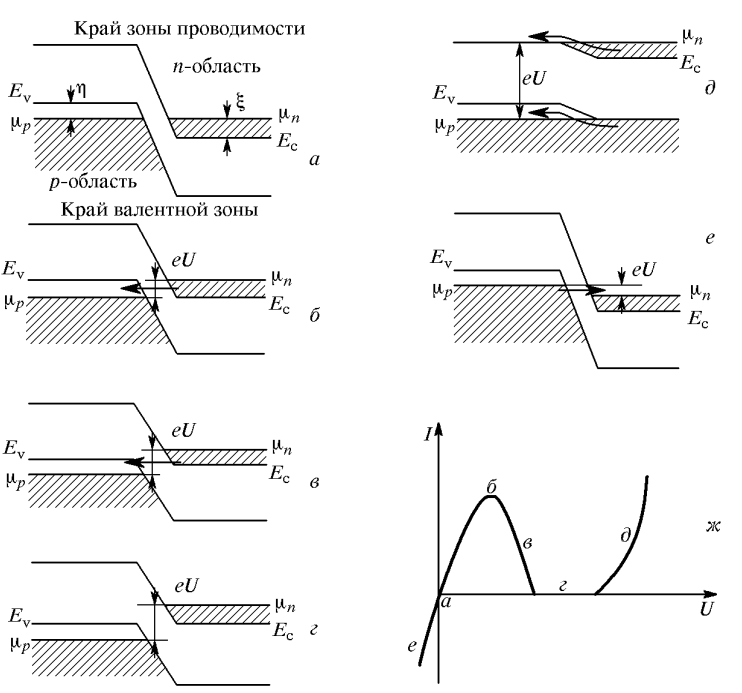
\includegraphics[width=0.48\textwidth]{fig1}
  \end{center}
  \caption{Схема энергетических уровней и вольт-амперная характеристика идеального туннельного диода}
\end{wrapfigure}

При малых уровнях легирования ($10^{14} - 10^{17} cm^{-3}$) полупроводник не вырожден, а уровень Ферми лежит в запрещенной зоне.Когда концентрация примеси превышает эффективные плотности состояний, уровень Ферми перемещается в валентную зону (в случае акцепторной примеси) либо в зону проводимости (для донорной примеси). Такой полупроводник считается вырожденным. В туннельном диоде качественно меняется вид электронного спектра полупроводника. У полупроводника n-типа на дне зоны проводимости появилась целая полоса, занятая электронами, а в полупроводнике p-типа образовалась полоса свободных состояний у потолка валентной зоны. Сильно легированный полупроводник стал полуметаллом. У всей системы образовался единый уровень Ферми -- единая граница свободных состояний.

В  сильно легированных полупроводниках в области узкого (p-n)-перехода становятся возможными туннельные переходы электронов, и поэтому такие диоды называются туннельными

Для того, чтобы туннельный ток при небольших напряжениях имел достаточную для измерения величину, необходимо, чтобы (p-n)-переход был достаточно узким и с обеих сторон перехода имелись изоэнергетические уровни, между которыми возможны туннельные переходы. Для этого как p-, так и n-области диода должны быть вырожденными

В вырожденном полупроводнике уровень Ферми лежит в разрешенной зоне, а в полупроводнике n-типа -- в зоне проводимости, в полупроводнике p-типа -- в валентной зоне.

Приложим к туннельному диоду внешнее поле в прямом направлении, т.е. минус к n-области, а плюс к p-области. В этом случае внешнее поле противоположному в (p-n)-переходе. По мере увеличения приложенного напряжения смещение зон уменьшается и часть занятый состояний в n-области перекрывается с незанятыми состояниями в p-области. Электроны туннелируют налево, ток возрастает пропорционально как вероятности туннелирования,так и плотности занятый состояний справа и незанятых состояний слева.

\begin{wrapfigure}{l}{0.5\textwidth}
  \begin{center}
    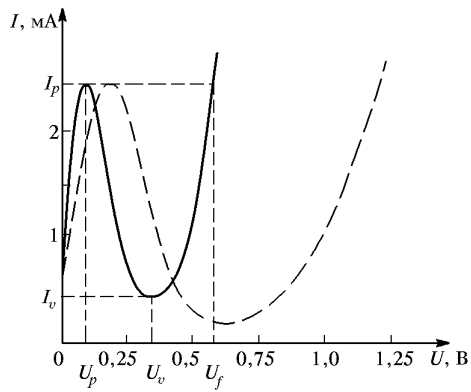
\includegraphics[width=0.48\textwidth]{fig2}
  \end{center}
  \caption{Экспериментальные вольт-амперные характеристики туннельных диодов при комнатной температуре: сплошная линия -- для германия, штриховая -- для диода из арсенида галлия}
\end{wrapfigure}

При дальнейшем увеличении внешней разности потенциалов перекрытие уровней справа и слева достигает максимума, и ток через диод максимален. Затем, когда дно зоны проводимости попадает в область запрещенной зоны слева -- ток прекращается.

При обратном включении, уровень Ферми в p-области смещается вверх относительно уровня в n-области на величину внешнего напряжения, в цепи пойдет ток в обратном направлении. Так получается вольт-амперная характеристика идеального туннельного диода (рис. 1ж)

Особенностью реальной вольт-амперной характеристики является наличие тока на участке между туннельной и диффузионной ветвями. Основной причиной отличиная от нуля тока $I_\nu$ является образование примесных зон из-за большой концентрации донорных центров. 

Если на такой (p-n)--переход подать прямое напряжение, то произойдет смещение зон. По достижении напряжения $U_v$ ток через диод минимален, что соответствует совпадению границ зоны проводимости и валентной зоны. Отсюда можно оценить положение уровней Ферми:

$$
	U_v = \frac{\xi + \eta}{e},
$$ 

где $\xi$ -- расстояние от уровня Ферми до дна зоны проводимости в n--полупроводнике, $\eta$ -- расстояние от уровня Ферми до потолка валентной зоны в p--полупроводнике.

Если оба полупроводника вырождены одинаково, что практически соответствует действительности, то

$$
	U_v = \frac{2\eta}{e} = \frac{2\xi}{e}
$$ 

Напряжению $U_p$ соответствует пик тока $I_p$, при котором смещение энергетических зон должно быть одинаково, тогда:

$$
	U_p \approx \frac{\xi - E_{n \ max}}{e}
$$

Напряжение $U_f$, характеризующее раствор вольт-амперной зарактеристики, определяется в основном шириной запрещенной зоны в полупроводниковых диодах

\newpage

\section*{Экспериментальная установка}

\begin{figure}[h!]
	\centering
	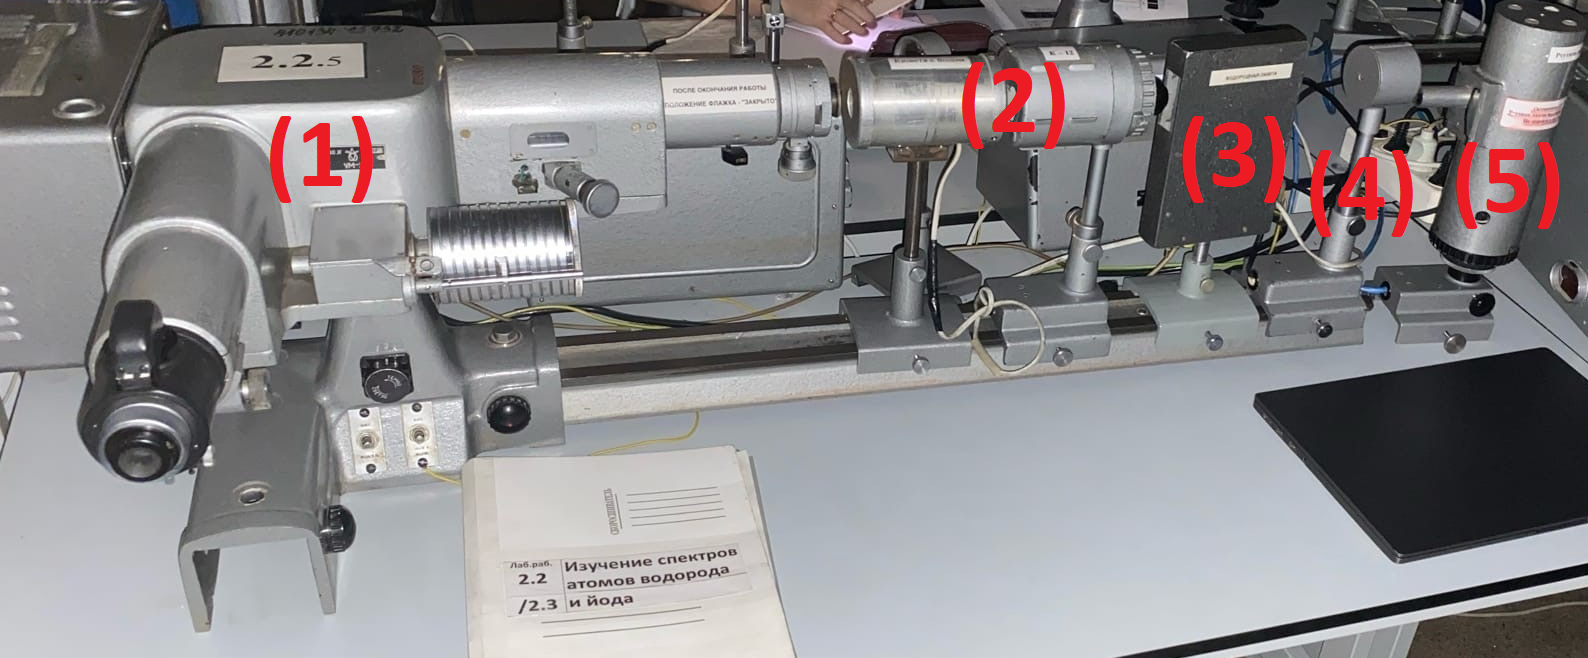
\includegraphics[width=\linewidth]{setup}
	\caption{Экспериментальная установка. (1) -- амперметр, (2) -- вольтметр, (3) -- звуковой генератор, (4) -- панель с элементами, (5) -- осциллограф}
\end{figure}

\begin{figure}[h!]
	\centering
	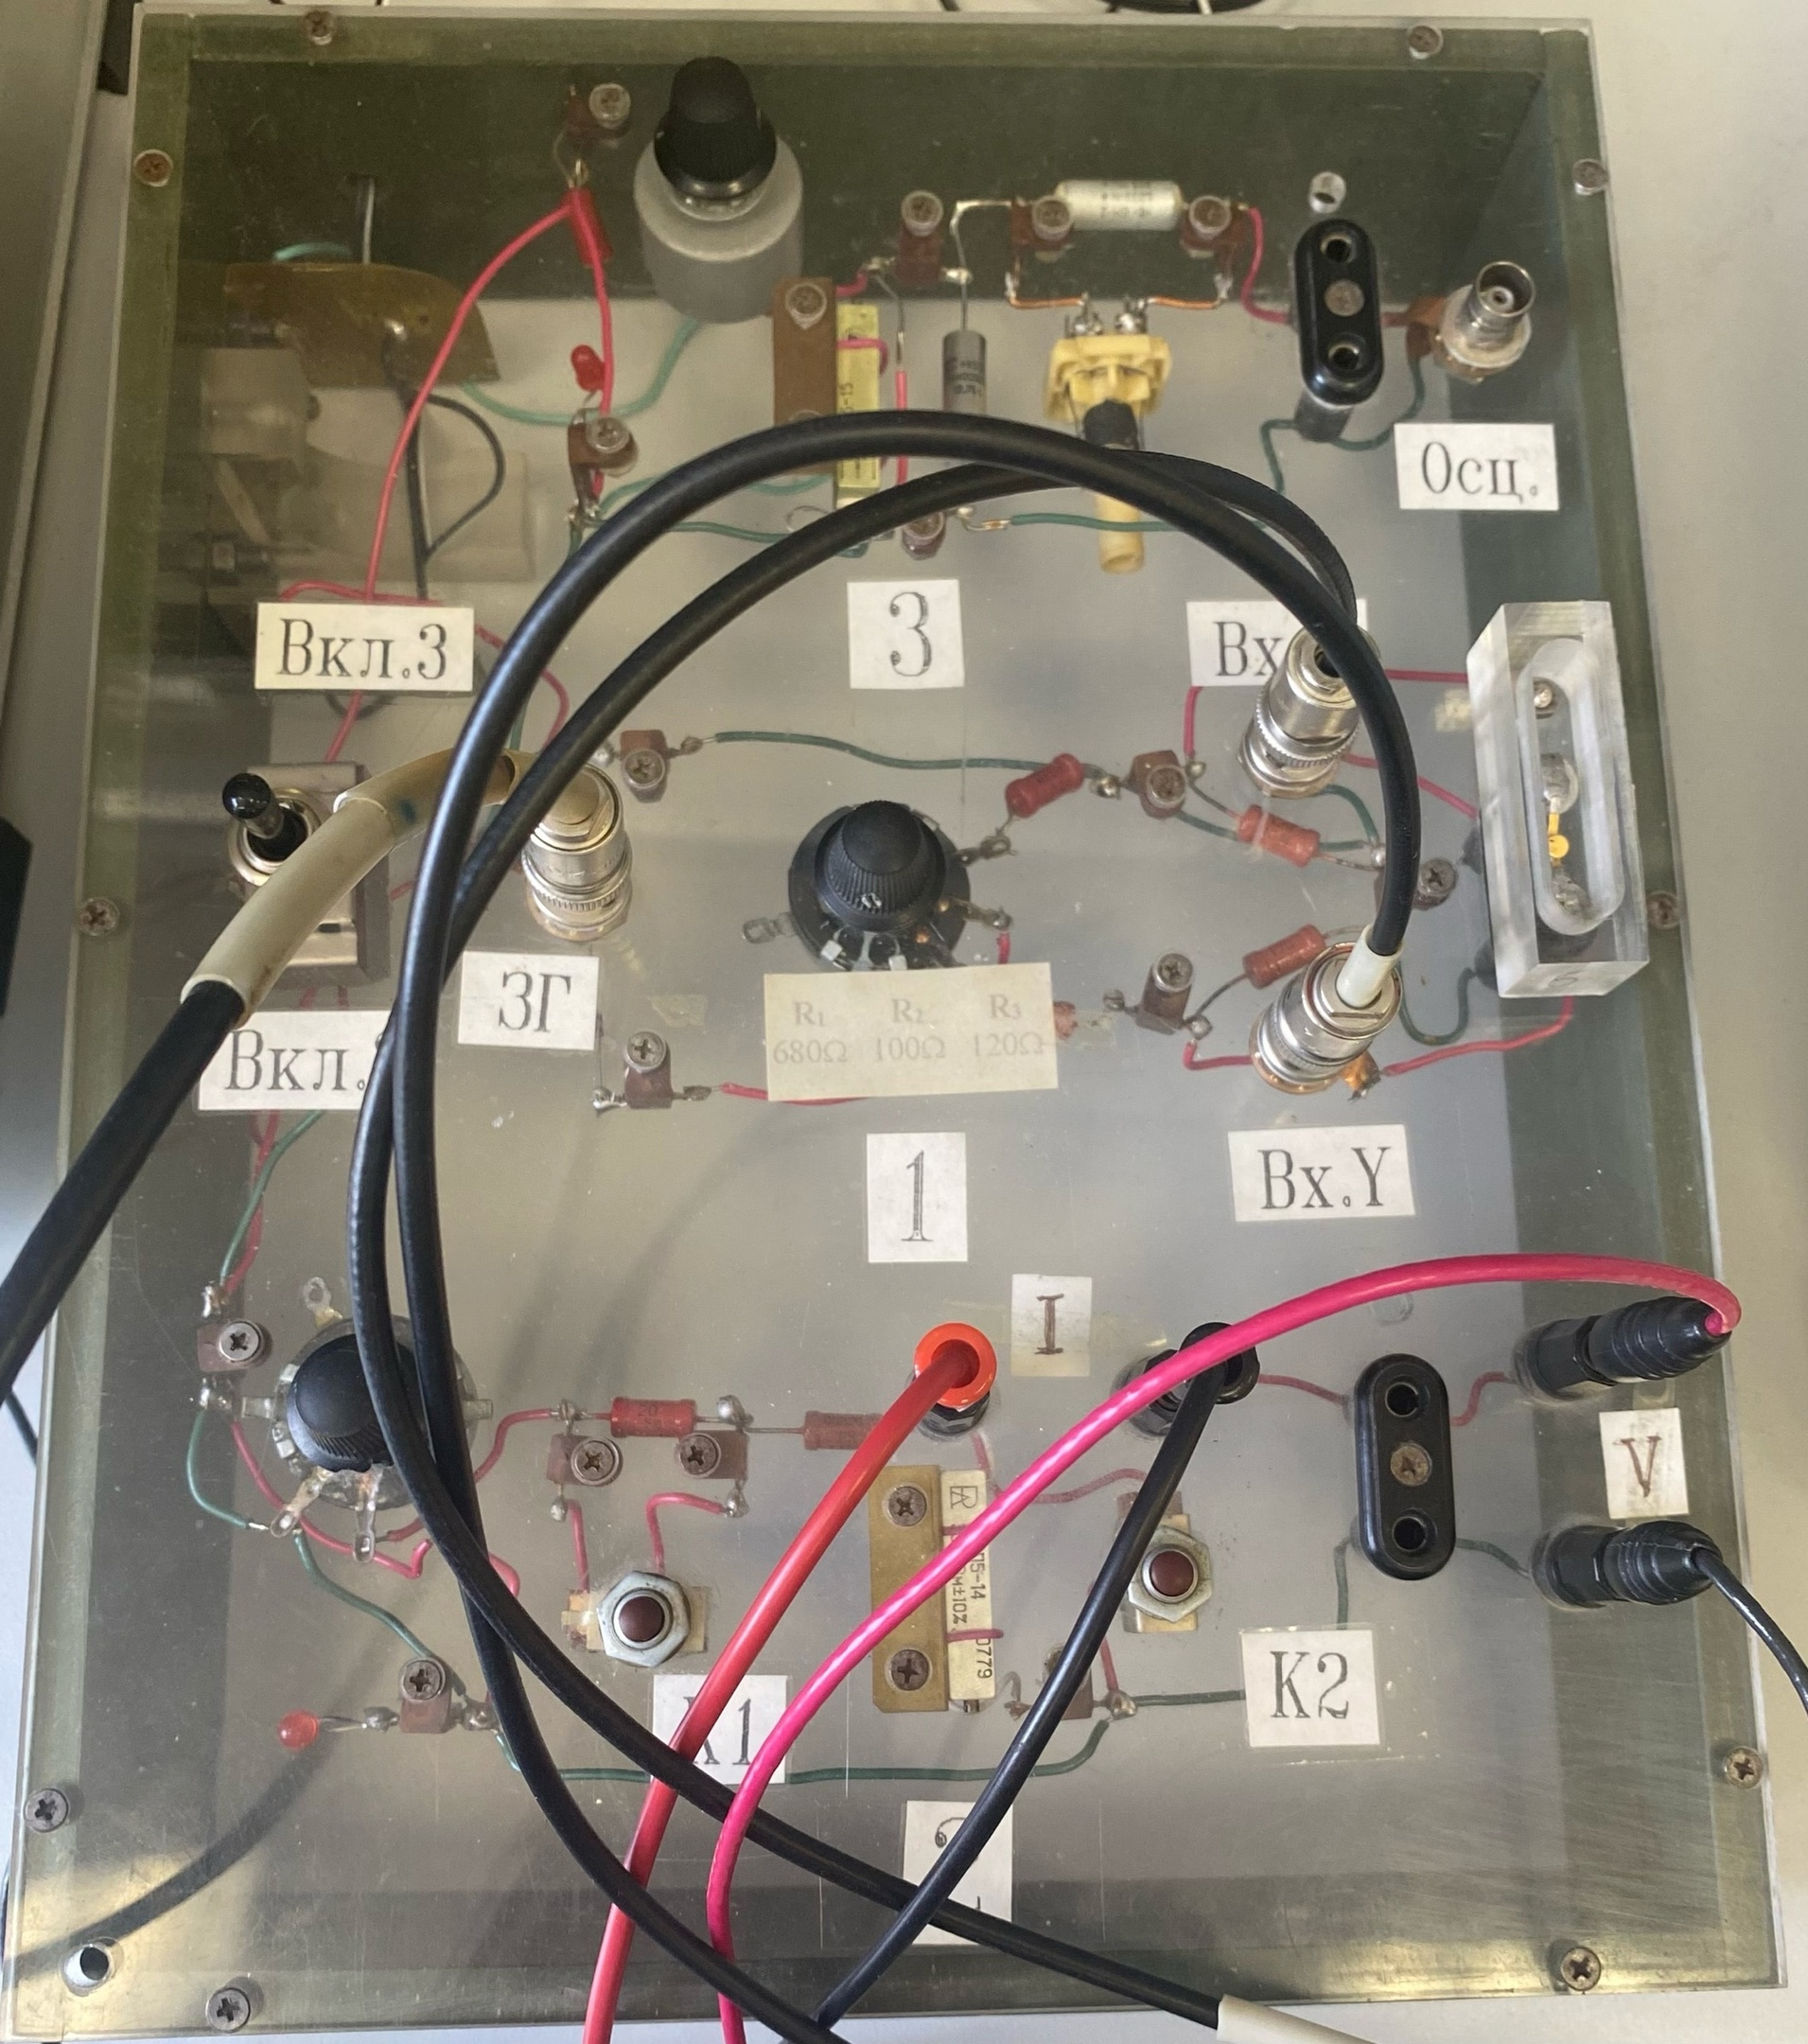
\includegraphics[scale=0.15]{plata}
	\caption{Панель с элементами. Переключатель <<Вкл.>> имеет 3 положения, соответствующие трем экспериментальным схемам}
\end{figure}

\section*{Ход работы}

\subsection*{Наблюдение вольт-амперной характеристики}

Поставим переключатель в среднее положение <<Вкл.>>, тогда электрическая схема имеет следующий вид

\begin{figure}[h!]
	\centering
	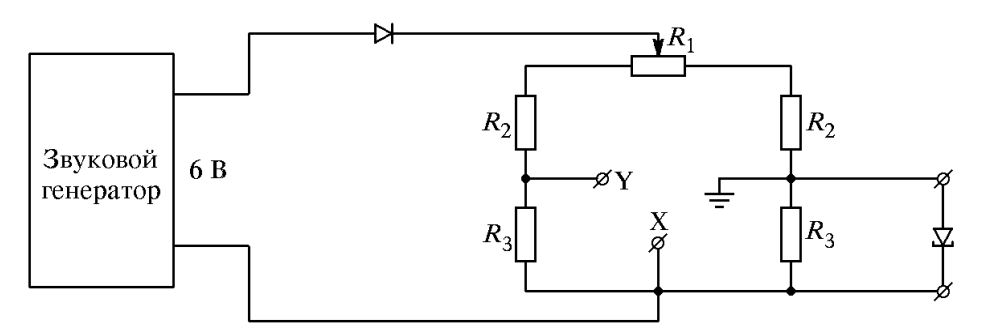
\includegraphics[width=\linewidth]{scheme_2}
	\caption{Принципиальная схема наблюдения вольт-амперной характеристики}
\end{figure}

После балансировки моста, получим вольт-амперную характеристику на экране осциллографа:

\begin{figure}[h!]
	\centering
	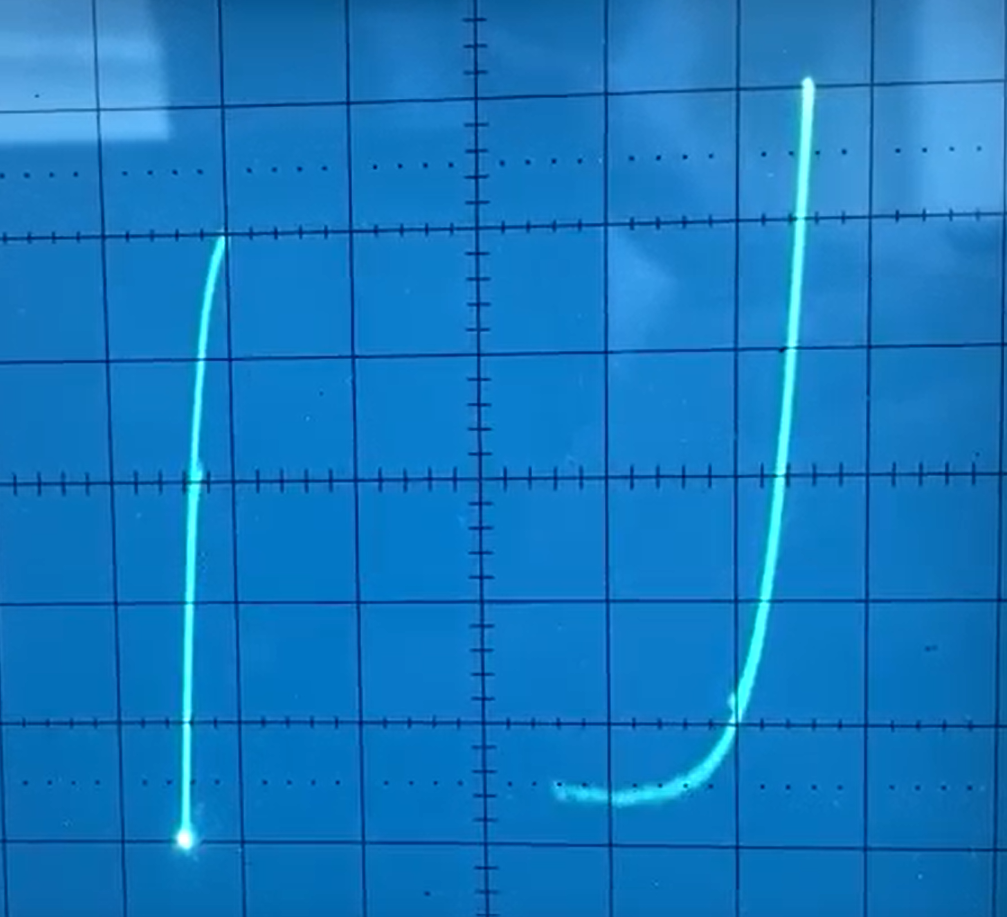
\includegraphics[width=0.5\linewidth]{osciloscope}
	\caption{Вольт-амперная характеристика туннельного диода}
\end{figure}

Измерим характерные значения напряжений 

\begin{align*}
	U_p = 0,05 \ В \\
	U_v = 0,36 \ В \\
	U_f = 0,52 \ В \\ 
\end{align*}

Оценим расстояние от уровня Ферми до дна зоны проводимости в n--полупроводнике $\xi$ и максимума распределение электронов в зоне проводимости $E_{n \ max}$:

\begin{align*}
	\xi &= \frac{eU_v}{2} \approx 0,18 \ эВ \\
	E_{n \ max} &= \xi - eU_p \approx 0,13 \ эВ \\
\end{align*}

\subsection*{Измерение вольт-амперной характеристики}

Поставим переключатель <<Вкл>> в нижнее положение, тогда электрическая схема имеет следующий вид:

\begin{figure}[h!]
	\centering
	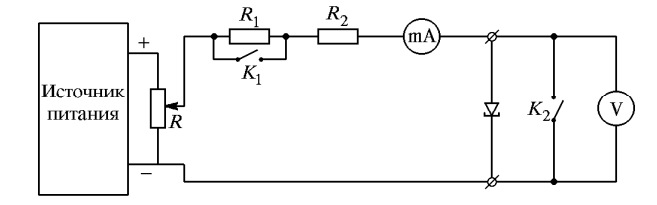
\includegraphics[width=\linewidth]{scheme_1}
	\caption{Принципиальная схема наблюдения вольт-амперной характеристики}
\end{figure}

Изменяя значения напряжения на диоде перемещением движка резистора R, получим вольт-амперную характеристику туннельного диода, данные занесем в Таблицу 1 

\begin{minipage}[c]{0.33\linewidth}
\begin{tabular}{|l|l|}
\hline
I, мА & U, В \\ \hline
0,011 & 0,000 \\ \hline
0,262 & 0,002 \\ \hline
0,443 & 0,003 \\ \hline
0,633 & 0,004 \\ \hline
0,810 & 0,005 \\ \hline
1,151 & 0,007 \\ \hline
1,467 & 0,009 \\ \hline
1,612 & 0,010 \\ \hline
1,765 & 0,011 \\ \hline
1,924 & 0,012 \\ \hline
2,082 & 0,013 \\ \hline
2,227 & 0,014 \\ \hline
2,404 & 0,015 \\ \hline
2,603 & 0,017 \\ \hline
2,736 & 0,018 \\ \hline
2,858 & 0,019 \\ \hline
0,399 & 0,360 \\ \hline
\end{tabular}
\end{minipage}
\begin{minipage}[c]{0.33\linewidth}
\captionof{table}{ВАХ диода}
\begin{tabular}{|l|l|}
\hline
I, мА & U, В \\ \hline
4,017 & 0,031 \\ \hline
4,233 & 0,034 \\ \hline
4,476 & 0,039 \\ \hline
2,409 & 0,265 \\ \hline
1,820 & 0,200 \\ \hline
1,808 & 0,191 \\ \hline
1,818 & 0,183 \\ \hline
1,902 & 0,214 \\ \hline
1,977 & 0,221 \\ \hline
2,081 & 0,229 \\ \hline
2,189 & 0,238 \\ \hline
2,292 & 0,249 \\ \hline
2,347 & 0,255 \\ \hline
2,433 & 0,269 \\ \hline
4,606 & 0,042 \\ \hline
0,399 & 0,342 \\ \hline
2,454 & 0,272 \\ \hline
\end{tabular}
\end{minipage}
\begin{minipage}[c]{0.33\linewidth}
\begin{tabular}{|l|l|}
\hline
I, мА & U, В \\ \hline
3,372 & 0,024 \\ \hline
3,677 & 0,027 \\ \hline
1,247 & 0,454 \\ \hline
1,777 & 0,467 \\ \hline
5,366 & 0,503 \\ \hline
2,507 & 0,479 \\ \hline
2,655 & 0,481 \\ \hline
4,555 & 0,498 \\ \hline
2,352 & 0,255 \\ \hline
2,439 & 0,269 \\ \hline
0,449 & 0,390 \\ \hline
0,423 & 0,379 \\ \hline
0,406 & 0,367 \\ \hline
0,623 & 0,420 \\ \hline
0,685 & 0,426 \\ \hline
\end{tabular}
\end{minipage}

\newpage

По полученным данным построим график 

\begin{figure}[h!]
	\centering
	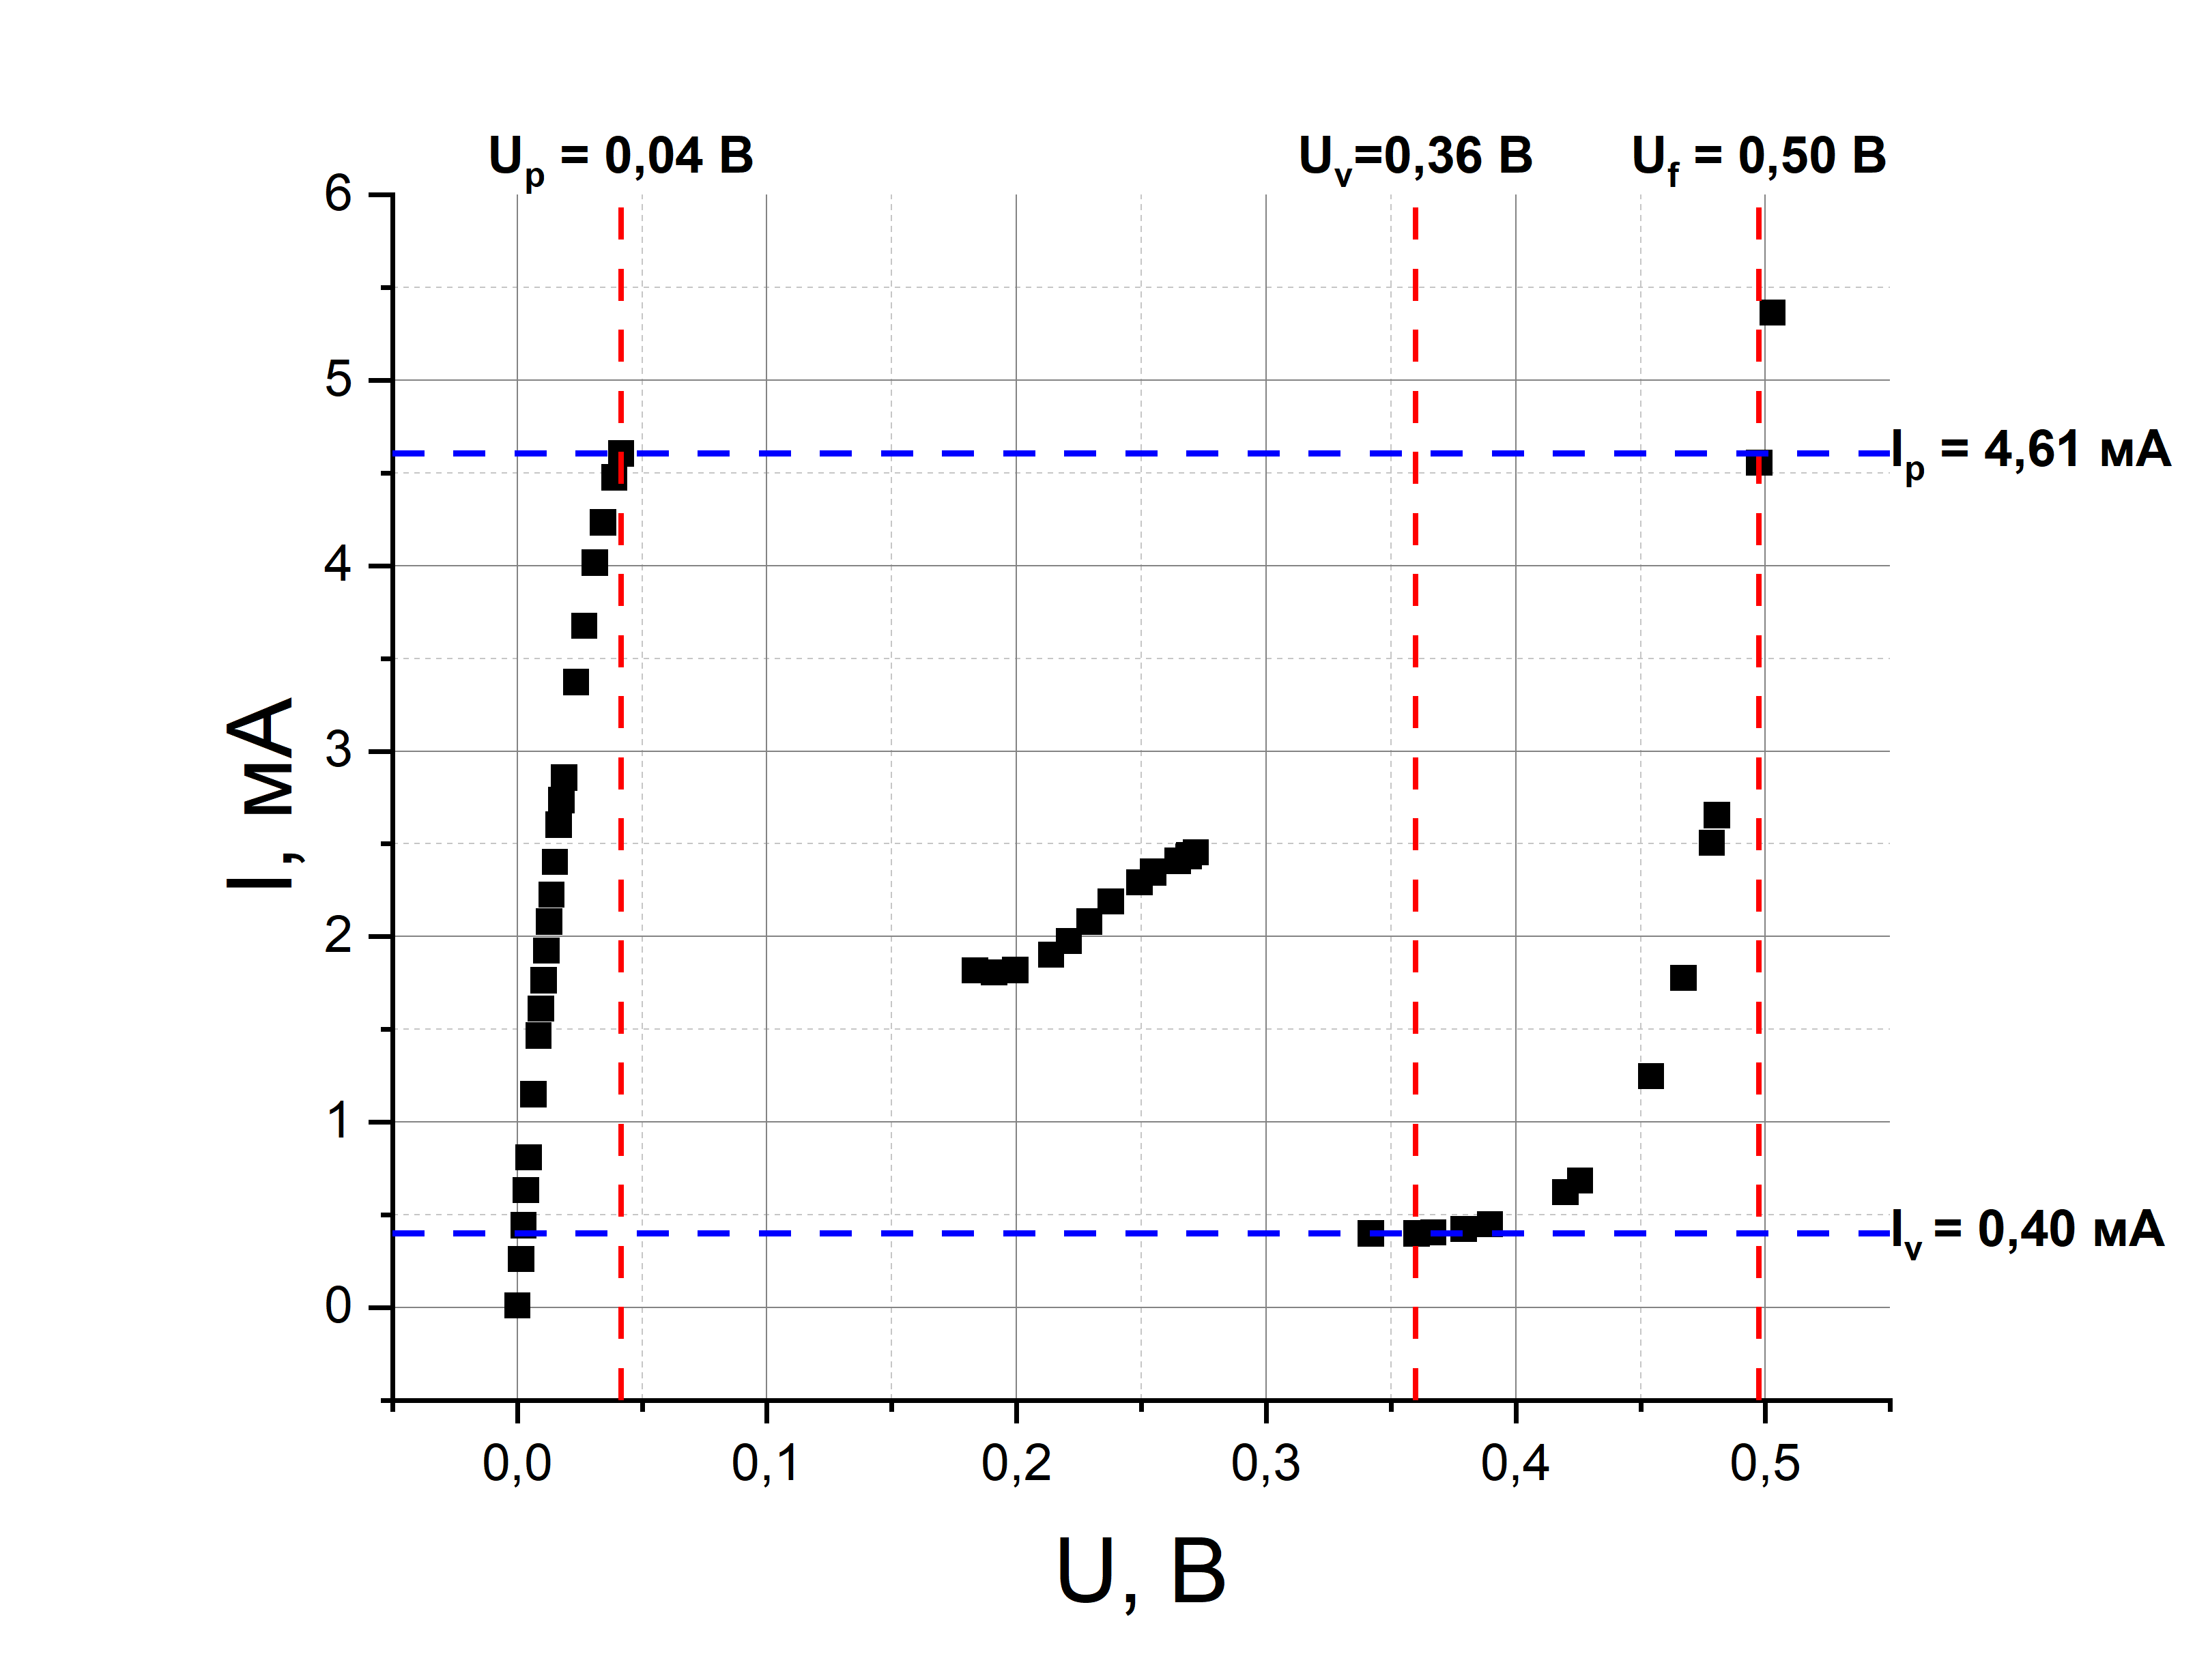
\includegraphics[width=\linewidth]{UI-characteristic}
	\caption{ВАХ туннельного диода}
\end{figure}

Из графика найдем характерные значения напряжений и токов:
\begin{align*}
	U_p = (400 \pm 1) \cdot 10^{-4} \ В \\
	U_v = (3600 \pm 1) \cdot 10^{-4} \ В \\
	U_f = (5000 \pm 1) \cdot 10^{-4} \ В \\
	I_p = (4,610 \pm 0,001) \ мА \\
	I_v = (0,040 \pm 0,001) \ мА \\ 
\end{align*}

Оценим расстояние от уровня Ферми до дна зоны проводимости в n--полупроводнике $\xi$ и максимума распределение электронов в зоне проводимости $E_{n \ max}$:

\begin{align*}
	\xi &= \frac{eU_v}{2} \approx (1800 \pm 1) \cdot 10^{-4} \ эВ \\
	E_{n \ max} &= \xi - eU_p \approx (1400 \pm 1) \cdot 10^{-4} \ эВ \\
\end{align*}

где погрешность $E_{n \ max}$ рассчитывалась по формуле:

$$
	\sigma_{E_{n \ max}} = \sqrt{ \sigma_{\xi}^2 + e^2 \sigma_{U_p}^2}
$$

\section*{Выводы}

В ходе работы были изучены основные характеристики туннельного диода:

\begin{itemize}
\item Была получена статическая картина ВАХ туннельного диода и, используя ее, были оценены параметры $\xi \approx 0,18 \ эВ$, $E_{n \ max} \approx 0,13 \ эВ$

\item Была получена зависимость тока через туннельный диод от приложенного к нему напряжения, используя эту зависимость была построена ВАХ туннельного диода и так же были оценены параметры: $\xi \approx 0,18 \ эВ$, $E_{n \ max} \approx 0,14 \ эВ$

\item Видно, что результаты полученные статическим и динамическим методами согласуются, что говорит о корректности проведения измерений
\end{itemize}

\end{document}